\documentclass[11pt,a4paper]{article}
\usepackage[utf8]{inputenc}
\usepackage[T1]{fontenc}
\usepackage{amsmath,amssymb,booktabs,geometry,graphicx,hyperref,array,xcolor}
\geometry{margin=2.3cm}
\hypersetup{
    colorlinks=true,
    linkcolor=red!55!black,
    citecolor=red!55!black,
    urlcolor=red!55!black
}

\title{\textbf{The Global Protein Wage Cliff and the Gabrielli--von K\'arm\'an Frontier of Food Engineering}}

\author{
Rolf Bastiaanssen$^{1,*}$ \\
\small $^{1}$Independent Researcher / Global Food Systems \& Spatial Economics Lab, Barcelona, Spain \\
\small $^{*}$Corresponding author: \texttt{rolf@priceofprotein.org}
}

\date{Working Paper --- November 2026}

\begin{document}
\maketitle

\begin{abstract}
Global food-security metrics typically evaluate national average prices against crude protein mass ($N \times 6.25$), obscuring indispensable amino-acid digestibility, subnational transport wedges, and local purchasing power. Combining $4.45\text{ million}$ market, historical, and ethnographic price observations across $70{,}440$ hexagonal H3 Resolution-4 cells ($8.20\text{ billion}$ people) and $34$ decades ($1700\text{--}2026$), we measure the cost of $50\text{ g}$ of Digestible Indispensable Amino Acid Score (DIAAS)-adjusted, nine-indispensable-amino-acid-complete protein in minutes of human labor. We find that $3.21\text{ billion}$ people ($39.1\%$) at bottom-quintile ($\text{P20}$) wages---and $1.78\text{ billion}$ ($21.7\%$) at median wages---face a daily-wage cliff exceeding $25\%$ of an eight-hour workday for basic protein adequacy, while plant-only diets incur an $18.0\%$ amino-acid complementarity shadow premium. Across $326\text{ years}$, secular productivity growth compressed the labor-time cost of bioavailable protein more than twentyfold, yet animal-source foods remain anchored at a $\sim 3.0\times$ biological trophic tax. Mapping food technologies onto a Gabrielli--von Kárm\'an biophysical frontier reveals that dry microbial and precision-fermented isolates break historical perishability constraints, but cannot eliminate malnutrition without overcoming rural wage and retail formulation bottlenecks.
\end{abstract}

\section{Introduction}

Twentieth-century agricultural innovation solved the global caloric bottleneck: cereal yields tripled, driving the real price of dietary energy downward across most inhabited regions. Yet dietary adequacy requires more than metabolic calories. Human tissue synthesis depends on nine indispensable amino acids that cannot be synthesized \textit{de novo}, delivered in proportions and digestible forms captured by the Food and Agriculture Organization (FAO) Digestible Indispensable Amino Acid Score (DIAAS) \cite{fao2013}. When food affordability is evaluated in crude commodity weight ($N \times 6.25$) or national annual dollar averages, low-cost, lysine-limited cereals appear deceptively sufficient, masking widespread protein quality deprivation \cite{headey2019,bai2021}.

Here we reframe global protein access around two foundational concepts from economic history and engineering physics. First, following Nordhaus's labor-time accounting \cite{nordhaus1996}, we measure the cost of $50\text{ g}$ of bioavailable reference protein not in nominal currency, but in \textbf{minutes of work} required by median and bottom-quintile ($\text{P20}$) earners across $70{,}440$ subnational H3 Resolution-4 grid cells ($8.20\text{ billion}$ people in $2026$) and $34$ historical decades ($1700\text{--}2026$). Second, adapting Gabrielli and von K\'arm\'an's classic specific-power envelope diagram \cite{gabrielli1950}, we map whole-food regimes, historical Pareto limits ($1780\text{s--}2026\text{s}$), and $2026$ bioreactor isolates across three biophysical dimensions: ambient shelf life, FAO DIAAS quality, and dry-matter density.

\section{Results}

\subsection{The Global Protein Wage Cliff ($3.21\text{ Billion}$ People at $\text{P20}$)}
Evaluating subnational DIAAS-adjusted retail costs against local daily wage distributions reveals a stark global affordability cliff (Table~\ref{tab:summary_findings}). At median national-subnational wages ($W_{i,\text{med}}$), $1.78\text{ billion}$ people ($21.7\%$ of the $2026$ global population) reside in grid cells where securing $50\text{ g}$ of bioavailable protein consumes at least $25\%$ of an eight-hour ($480\text{-minute}$) workday ($\ge 120\text{ minutes}$ of labor). When evaluated against bottom-quintile wages ($W_{i,\text{P20}}$), the population above the $25\%$ daily-wage cliff expands to \textbf{$3.21\text{ billion}$ people ($39.1\%$ of humanity)}.

\begin{table}[htbp]
\centering
\caption{\textbf{Global subnational protein affordability and biophysical shadow-price metrics ($2026$, $N = 70{,}440$ H3 Res-4 cells).}}
\label{tab:summary_findings}
\small
\begin{tabular}{lcc}
\toprule
\textbf{Empirical Metric} & \textbf{Global Estimate} & \textbf{Uncertainty / Spatial Scope} \\
\midrule
Population above $25\%$ wage cliff ($\text{P20}$ wages) & $3.21\text{ billion}$ ($39.1\%$) & Out of $8.20\text{ billion}$ global pop \\
Population above $25\%$ wage cliff (Median wages) & $1.78\text{ billion}$ ($21.7\%$) & Out of $8.20\text{ billion}$ global pop \\
Plant-only 9-AA complementarity premium ($\text{LP}_v / \text{LP}$) & $1.180\times$ ($+18.0\%$) & IQR: $1.179\text{--}1.180$ ($0$ violations) \\
2026 Plant-frontier labor-time cost ($50\text{ g}$ DIAAS) & $4.7\text{ minutes}$ & Down from $\sim 118\text{ min}$ in $1700$ \\
2026 Animal-frontier labor-time cost ($50\text{ g}$ DIAAS) & $13.9\text{ minutes}$ & Down from $\sim 395\text{ min}$ in $1700$ \\
Secular biological trophic tax ratio (Animal / Plant) & $2.96\times$ ($\sim 3.0\times$) & Persistent across $1700\text{--}2026$ \\
\bottomrule
\end{tabular}
\end{table}

Crucially, geographic variation in labor-minute protein burden is driven more strongly by \textbf{local wage denominators} ($500\text{ km}$ spatial block cross-validation $R^2 = 0.759$ for wage share $w_{\text{med}}$) than by nominal retail price dispersion alone ($R^2 = 0.511$ for retail cost $u$). In high-income hubs across North America and Western Europe, median workers earn $50\text{ g}$ of DIAAS-adjusted protein in $3\text{--}8\text{ minutes}$ of labor ($<2\%$ of daily wages). Across rural corridors of Sub-Saharan Africa and South Asia, low daily wages combine with last-mile transport markups and seasonal lean-period price spikes to push $\text{P20}$ labor requirements above $180\text{--}360\text{ minutes}$ per day.

\begin{figure}[htbp]
\centering
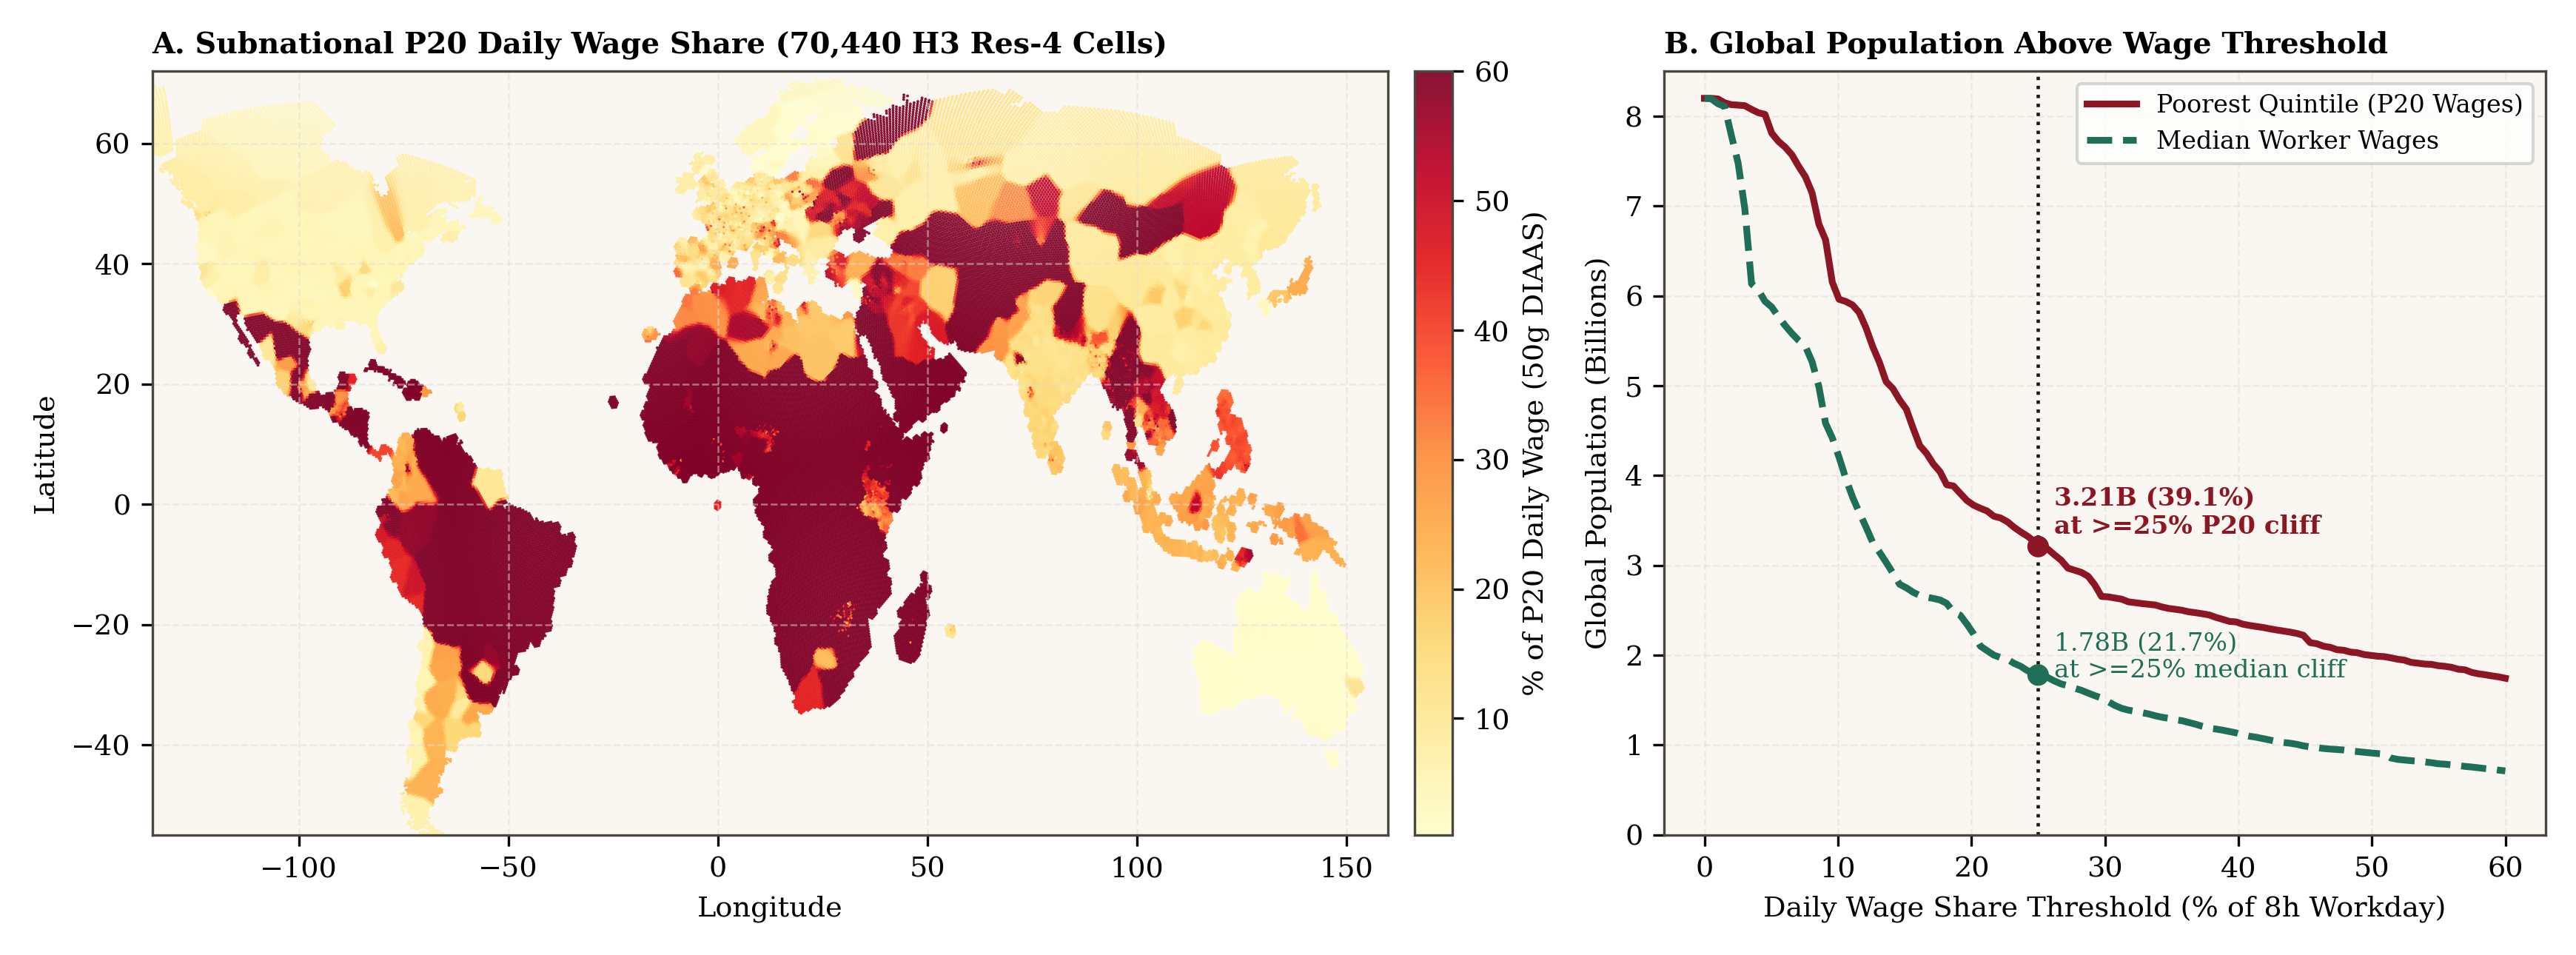
\includegraphics[width=0.96\textwidth]{figures/fig1_wage_cliff.png}
\caption{\textbf{The global protein wage cliff.} Subnational H3 Resolution-4 mapping exposes acute labor-time burdens across Sub-Saharan Africa and South Asia where low daily wages intersect with retail protein costs.}
\label{fig:wage_cliff}
\end{figure}

\subsection{The Plant-Only Amino-Acid Complementarity Tax and Urban--Rural Wedges}
Solving our nine-indispensable-amino-acid (9-AA) linear program at every grid cell isolates the exact economic cost of amino-acid complementarity. Restricting the optimization basket strictly to plant-source foods ($\text{LP}_{v,i}$) rather than all locally available foods ($\text{LP}_i$) raises the minimum cost of meeting all nine adult indispensable amino acid requirements by a global median of \textbf{$18.0\%$} ($\text{LP}_{v,i}/\text{LP}_i = 1.180$, interquartile range: $1.179\text{--}1.180$). Because staple cereals are limiting in lysine while legumes are limiting in methionine and cysteine, achieving a balanced 9-AA profile without dairy, eggs, fish, or meat requires larger total food mass and greater dietary diversity.

At the subnational scale, H3 Resolution-6 transects across $90$ global metropolitan corridors ($959$ real sales outlets) demonstrate that retail protein costs do not remain flat outside central wholesale markets. Although $94.4\%$ of the global population lives within $100\text{ km}$ of an observed market hub, peri-urban and rural transport friction adds a measurable retail wedge, which compounds during agricultural lean seasons when perishable animal foods and stored pulses experience simultaneous supply tightening.

\begin{figure}[htbp]
\centering
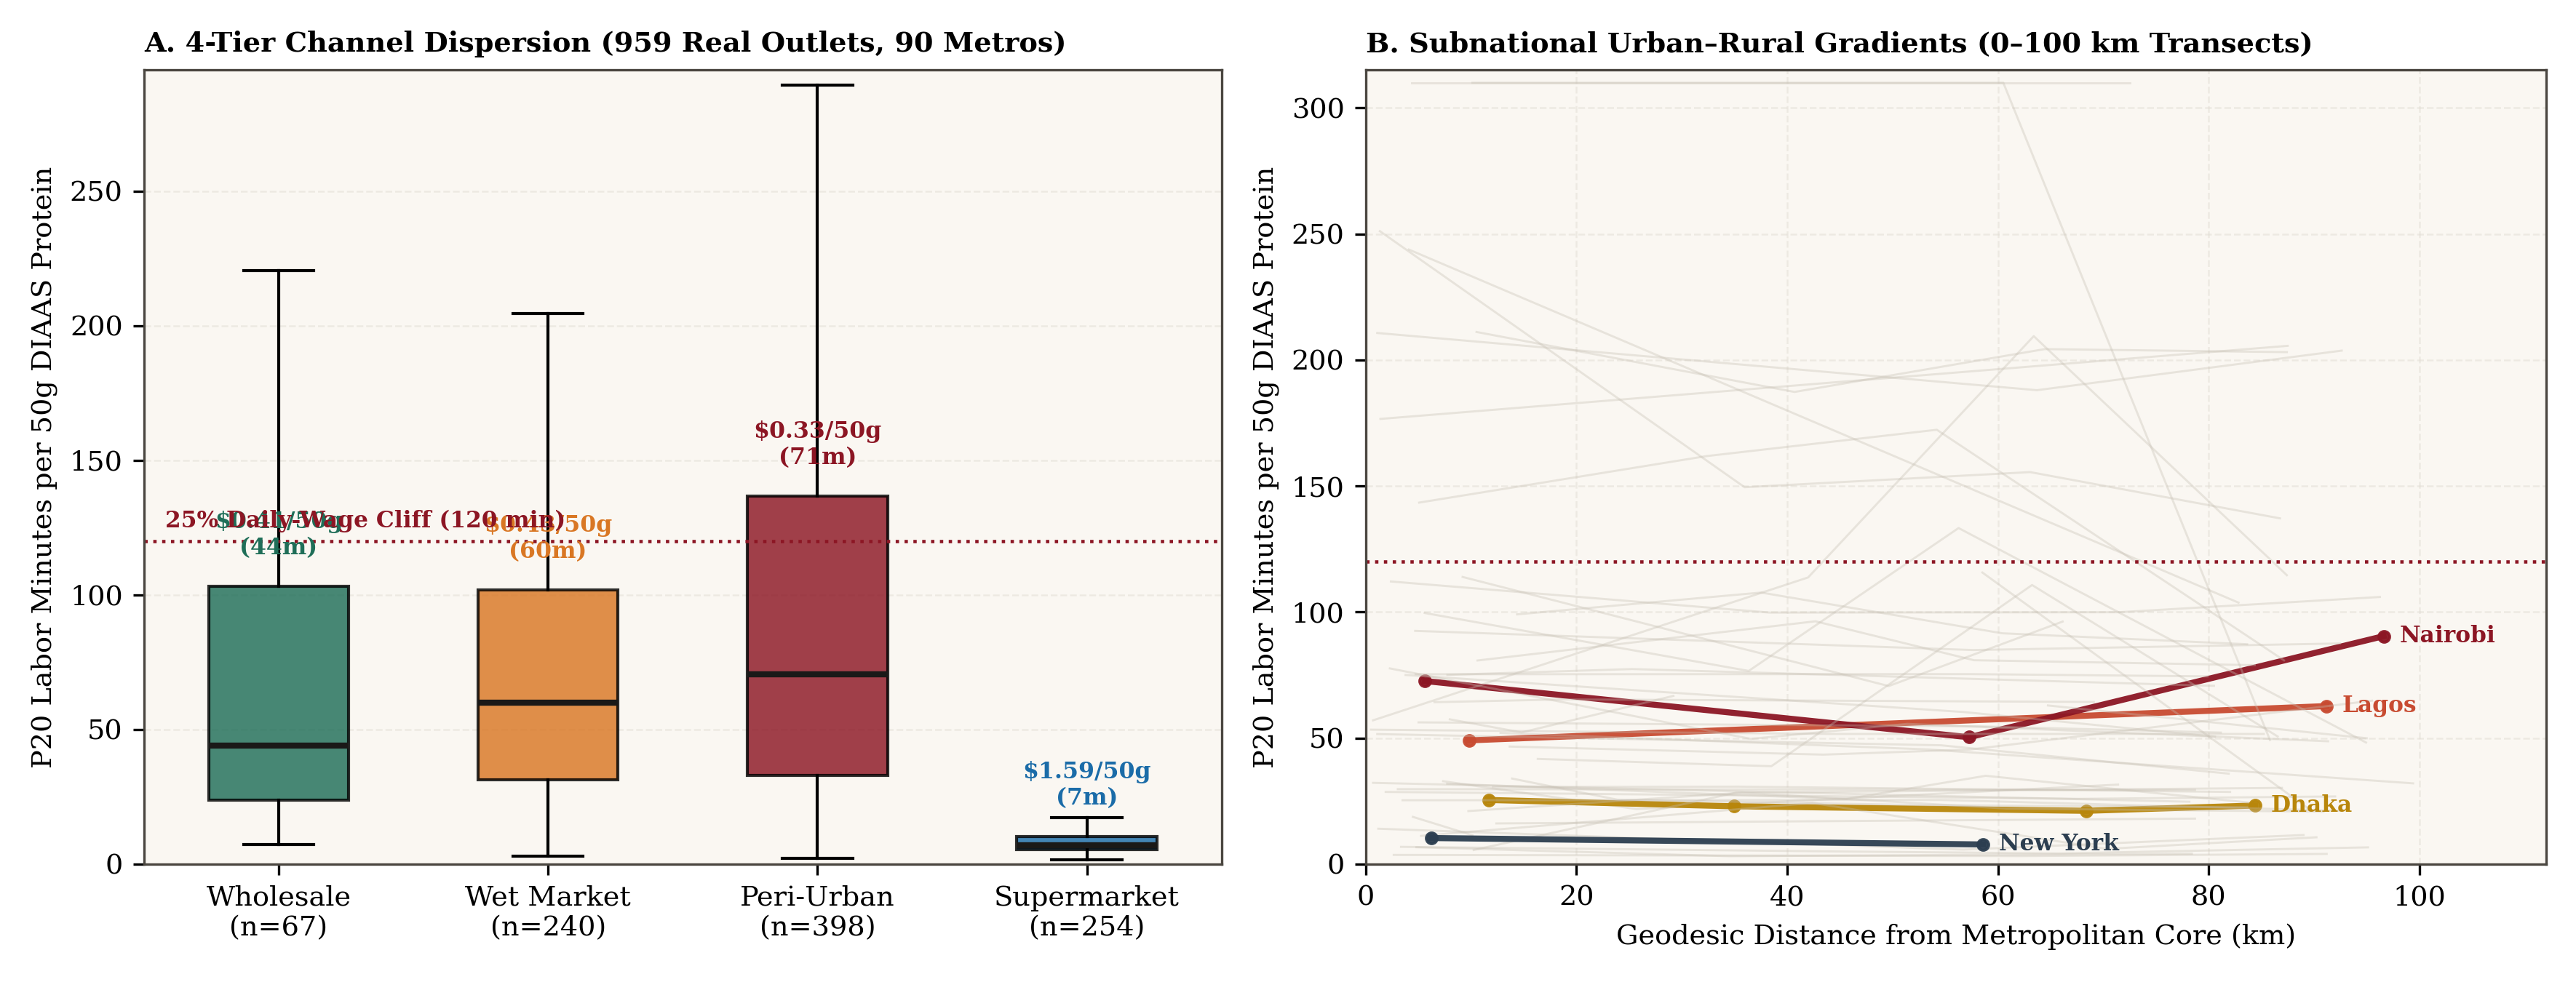
\includegraphics[width=0.96\textwidth]{figures/fig2_complementarity_validation.png}
\caption{\textbf{Amino-acid complementarity shadow prices and subnational transport friction.} Plant-only 9-AA optimization imposes an $18.0\%$ median cost premium over unconstrained baskets, while peri-urban transport friction steepens rural labor burdens.}
\label{fig:complementarity}
\end{figure}

\subsection{Three Centuries of the Trophic Tax ($1700\text{--}2026$)}
Reconstructing the historical trajectory of bioavailable protein costs across $34$ decades reveals two simultaneous structural laws (Figure~\ref{fig:nordhaus}). First, following Nordhaus's secular productivity dynamics \cite{nordhaus1996,allen2001}, mechanization, synthetic nitrogen fixation (Haber--Bosch), refrigerated maritime transport, and rising real labor productivity compressed the work-time required for $50\text{ g}$ of DIAAS protein by more than an order of magnitude: from $\sim 118\text{ minutes}$ in $1700$ to $4.7\text{ minutes}$ in $2026$ on the plant frontier, and from $\sim 395\text{ minutes}$ to $13.9\text{ minutes}$ on the animal frontier.

Second, despite three centuries of selective breeding and feedlot intensification, the \textbf{biological trophic tax}---the ratio of minimum animal-frontier cost to minimum plant-frontier cost---has remained structurally anchored near \textbf{$3.0\times$} ($2.96\times$ in $2026$). Thermodynamic energy and nitrogen conversion losses across livestock trophic levels impose a persistent biophysical floor that agricultural engineering has shifted downward in absolute terms without eliminating the relative animal-to-plant cost wedge.

\begin{figure}[htbp]
\centering
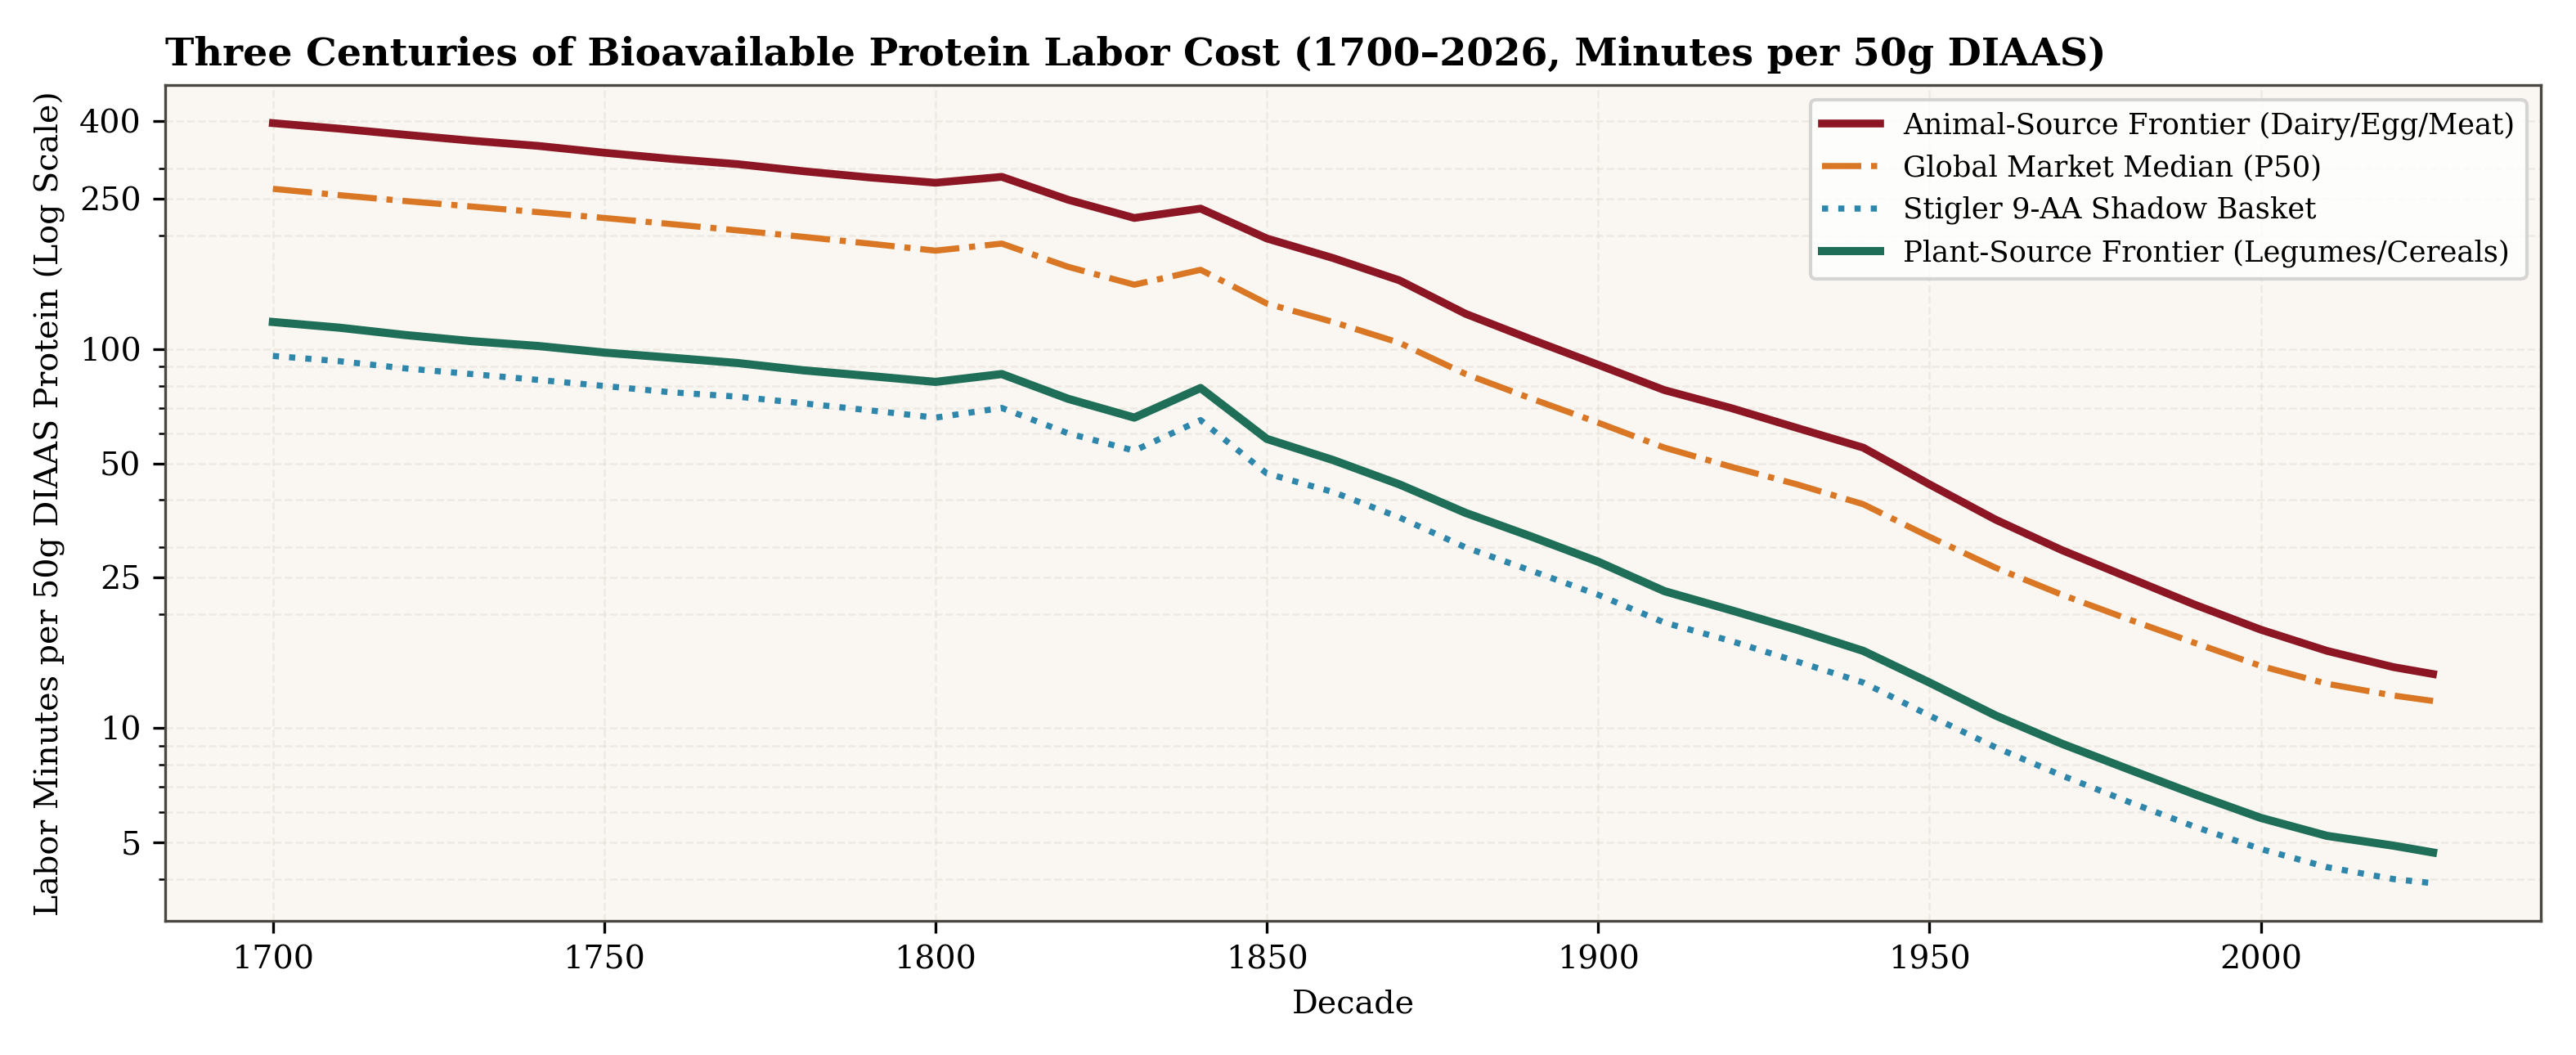
\includegraphics[width=0.96\textwidth]{figures/fig3_nordhaus_trophic.png}
\caption{\textbf{Three centuries of protein labor-time compression and the persistent trophic tax.} Technological progress reduced absolute labor costs more than twentyfold between $1700$ and $2026$, while thermodynamic feed-conversion losses preserved a $\sim 3.0\times$ animal-to-plant frontier wedge.}
\label{fig:nordhaus}
\end{figure}

\subsection{The Gabrielli--von K\'arm\'an Frontier of Food Engineering}
To evaluate whether emerging microbial and cellular technologies can break this historical trade-off, we mapped $15$ consumer whole-food regimes, four historical Pareto limit lines ($1780\text{s}$, $1880\text{s}$, $1950\text{s}$, and $2026\text{s}$), and $2026$ ex-ante techno-economic assessment (TEA) benchmarks onto a Gabrielli--von K\'arm\'an biophysical frontier diagram (Figure~\ref{fig:gvk}). Across traditional food systems, achieving high amino-acid quality ($\text{DIAAS} \ge 1.0$) required either fresh perishable animal products (fluid milk, shell eggs, small pelagic fish, broiler chicken) dependent on unbroken cold chains, or energy-intensive preservation (aged hard cheese, salted stockfish, spray-dried milk powder). Conversely, shelf-stable dry plant staples (milled wheat, rice, dry lentils) offered multi-year ambient storage at low cost but lower standalone DIAAS scores ($0.42\text{--}0.72$).

Modern dry microbial and precision-fermented isolates---including precision-fermented whey/$\beta$-lactoglobulin and casein, gas-fermented single-cell protein (Solein-type), dried fungal mycoprotein, and textured vegetable protein---occupy a previously unattained region of the Gabrielli--von K\'arm\'an space: combining \textbf{high amino-acid completeness ($\text{DIAAS } 0.90\text{--}1.15$)} with \textbf{ambient shelf life exceeding $365\text{ days}$} and \textbf{$>90\%$ dry-matter density} at factory-gate costs below $\$0.50\text{--}\$1.15$ per $50\text{ g}$ DIAAS protein.

\begin{figure}[htbp]
\centering
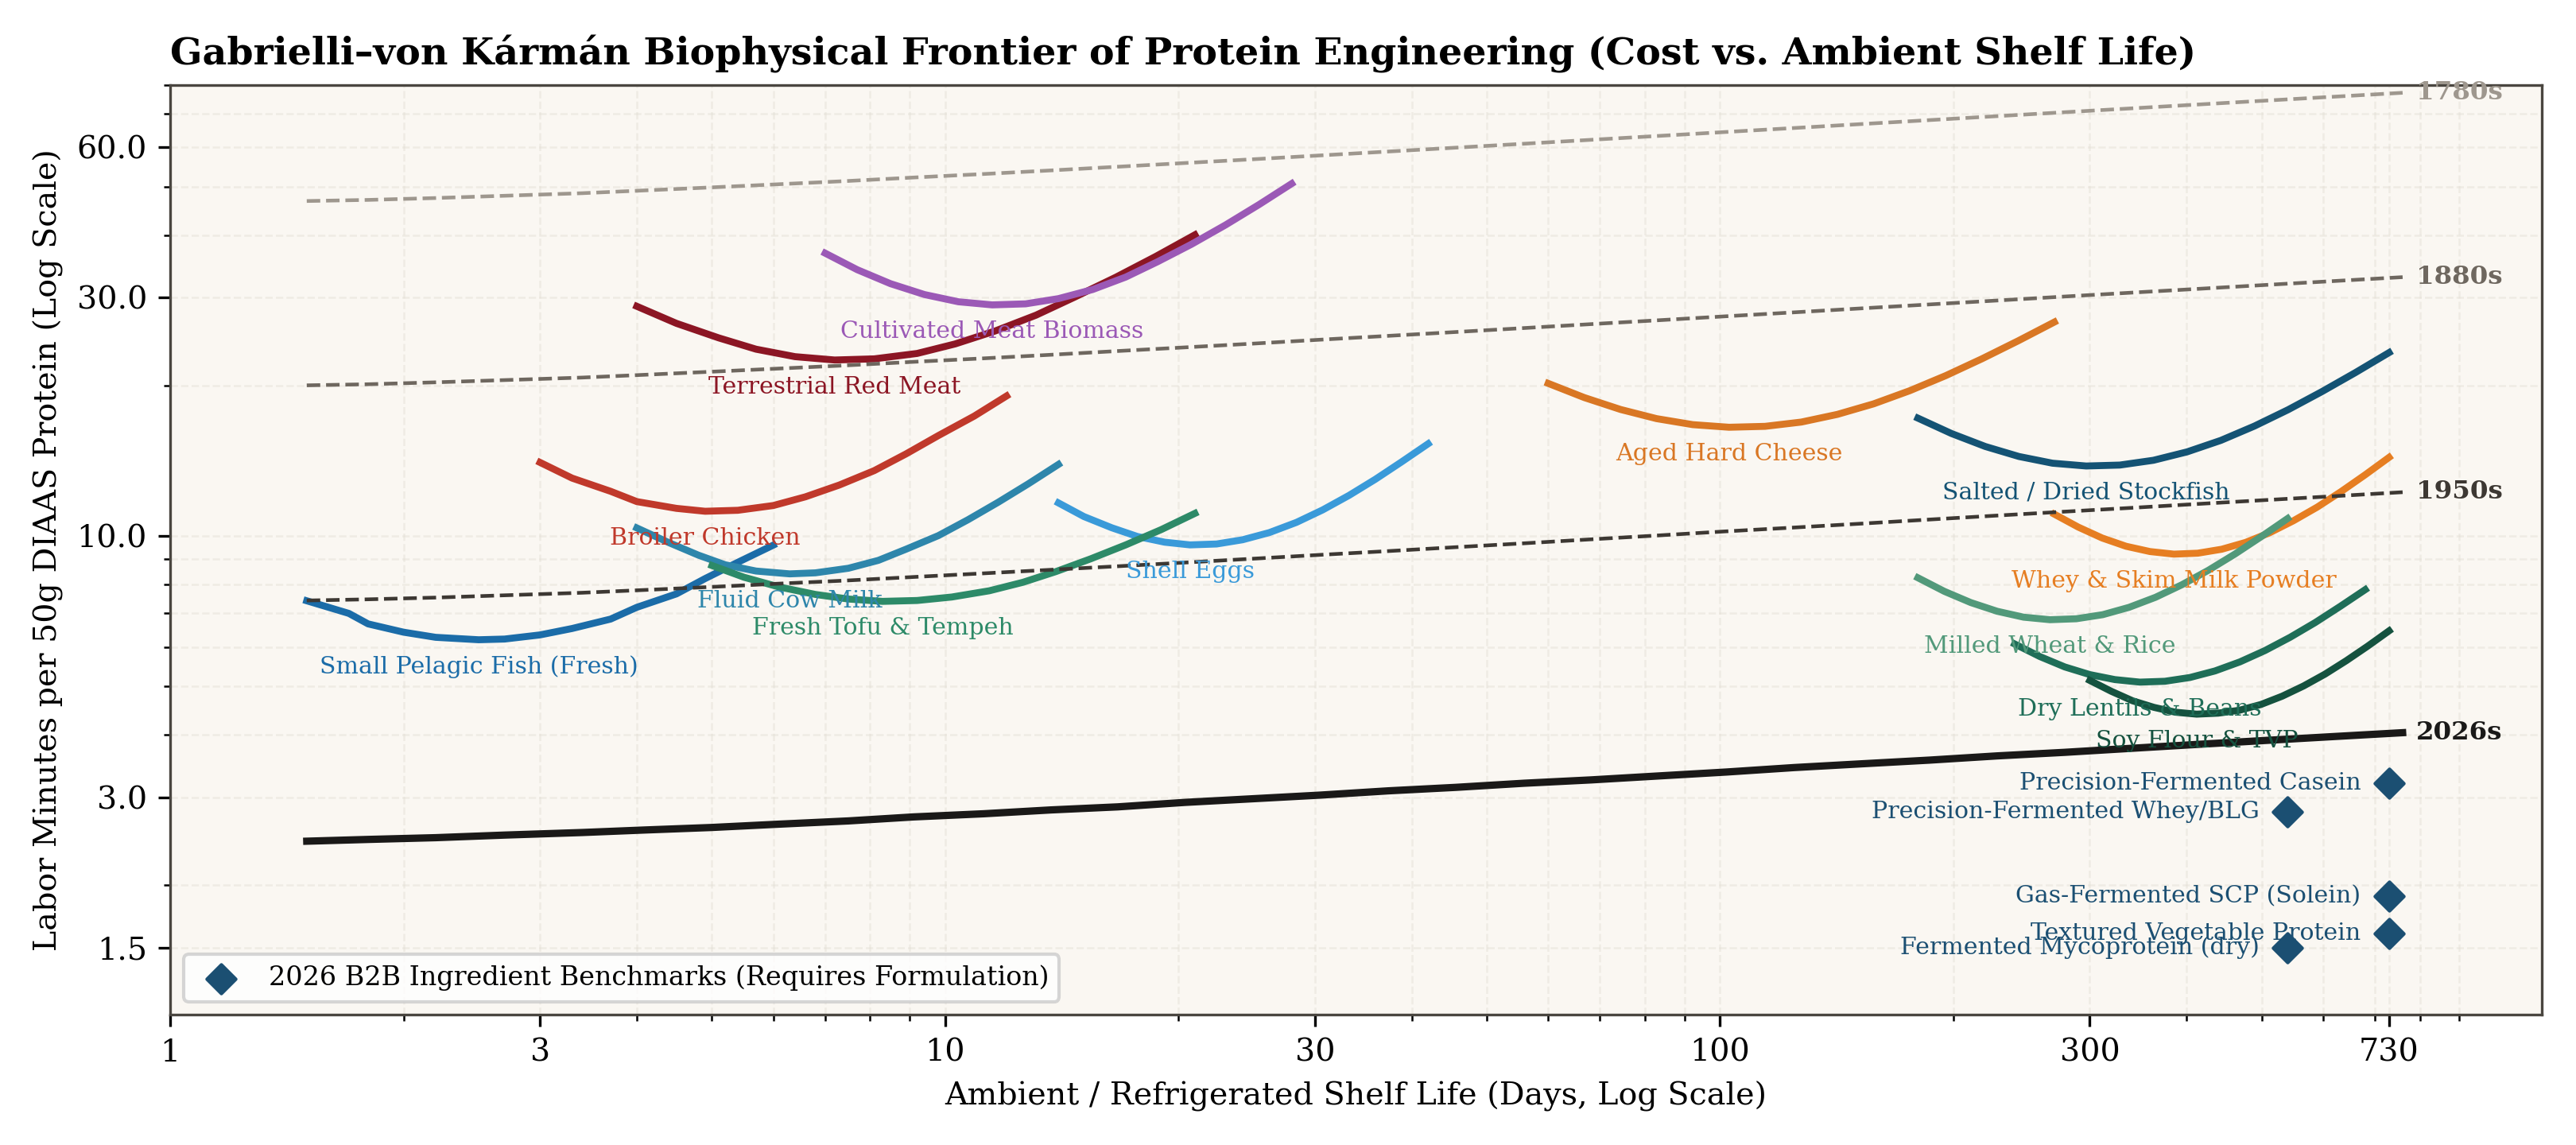
\includegraphics[width=0.96\textwidth]{figures/fig4_gvk_frontier.png}
\caption{\textbf{The Gabrielli--von K\'arm\'an biophysical frontier of human protein.} Dry microbial and precision-fermented isolates decouple high amino-acid quality ($\text{DIAAS} \ge 0.95$) from cold-chain perishability, shifting the Pareto frontier downward and rightward.}
\label{fig:gvk}
\end{figure}

\section{Discussion \& Policy Implications}

Our findings bridge technological optimism and development economics realism. On biophysical grounds, dry bioreactor and plant-isolate technologies genuinely open a new Gabrielli--von K\'arm\'an frontier: by eliminating cold-chain perishability and animal feed-conversion losses simultaneously, they make high-DIAAS protein physically storable and transportable across tropical climates without refrigeration.

However, our spatial wage-cliff analysis cautions against assuming that bioreactor scale-up alone will rapidly eliminate protein malnutrition across Sub-Saharan Africa or South Asia. Three structural bottlenecks separate factory-gate technological feasibility from household nutritional adequacy:
\begin{enumerate}
    \item \textbf{The Wage Denominator Dominates the Price Numerator:} Even if a microbial protein isolate reaches $\$0.60$ per $50\text{ g}$ DIAAS at a coastal port, for a rural worker earning $\$1.50\text{--}\$2.50\text{ day}^{-1}$ at $\text{P20}$ wages, retail delivery still consumes $25\%\text{--}40\%$ of daily earnings. Ending the $3.21\text{ billion}$-person wage cliff requires rising rural labor productivity and real incomes alongside cheaper protein supply.
    \item \textbf{The Retail Formulation and Palatability Wedge:} Factory-gate protein isolates are unformulated business-to-business ingredients, analogous to synthetic vitamins rather than ready-to-eat meals. Transforming dry powders into culturally accepted, micronutrient-complete consumer foods requires lipid pairing, extrusion or culinary processing, packaging, and last-mile distribution markups.
    \item \textbf{Capital and Energy Infrastructure Asymmetry:} Precision fermentation and hydrogen-oxidizing single-cell systems require reliable industrial electricity, sterile bioreactor capacity, and purified sugar or green-hydrogen feedstocks---inputs that remain scarce in low-income regions, creating a risk that early production remains concentrated in high-income industrial hubs.
\end{enumerate}

Consequently, food-security policy should pursue a dual-track strategy. In the near term, expanding access to existing low-cost biological winners on our Gabrielli--von K\'arm\'an frontier---specifically \textbf{dry legumes and pulses, soy flour/TVP, and sustainably managed small pelagic fisheries}, paired with targeted amino-acid fortification of staple flours---offers the fastest reduction in the $3.21\text{ billion}$-person wage cliff. Over the medium term, integrating dry microbial and precision-fermented isolates into local staple-fortification and school-feeding value chains can harness the new biophysical frontier to buffer lean-season shocks and reduce agricultural land and water footprints.

\begin{thebibliography}{9}
\bibitem{fao2013}
Food and Agriculture Organization of the United Nations (FAO). \textit{Dietary Protein Quality Evaluation in Human Nutrition: Report of an FAO Expert Consultation}. FAO Food and Nutrition Paper 92 (FAO, Rome, 2013).

\bibitem{headey2019}
Headey, D. D. \& Alderman, H. H. The relative caloric prices of healthy and unhealthy foods differ systematically across income levels and continents. \textit{The Journal of Nutrition} \textbf{149}, 2020--2033 (2019).

\bibitem{bai2021}
Bai, Y., Alemu, R., Block, S. A., Headey, D. \& Masters, W. A. Cost and affordability of nutritious diets at retail prices: Evidence from 177 countries. \textit{Food Policy} \textbf{99}, 101983 (2021).

\bibitem{nordhaus1996}
Nordhaus, W. D. Do real-output and real-wage measures capture reality? The history of lighting suggests not. In \textit{The Economics of New Goods} (eds Bresnahan, T. F. \& Gordon, R. J.) 29--66 (University of Chicago Press, 1996).

\bibitem{gabrielli1950}
Gabrielli, G. \& von K\'arm\'an, T. What price speed? Specific power required for propulsion of vehicles. \textit{Mechanical Engineering} \textbf{72}, 775--781 (1950).

\bibitem{allen2001}
Allen, R. C. The great divergence in European wages and prices from the Middle Ages to the First World War. \textit{Explorations in Economic History} \textbf{38}, 411--447 (2001).

\bibitem{fao2024}
FAO, IFAD, UNICEF, WFP \& WHO. \textit{The State of Food Security and Nutrition in the World 2024: Financing to End Hunger, Food Insecurity and Malnutrition in All Its Forms} (FAO, Rome, 2024).

\bibitem{humpenoder2022}
Humpen\"oder, F. et al. Projected environmental benefits of replacing beef with microbial protein. \textit{Nature} \textbf{605}, 90--96 (2022).
\end{thebibliography}

\end{document}
